\subsubsection{\stid{1.09} Distributed Tasking at Exascale: PaRSEC}


\paragraph{Overview}

The PaRSEC Environment provides a runtime component to dynamically execute on
heterogeneous distributed systems, and a productivity toolbox that comprises a
development framework for the support of multiple domain specific languages
(DSLs) and extensions, with debugging, trace collection, and analysis tools.
%
The PaRSEC project team is dedicated to solving two challenging and
interdependent problems facing the ECP developer community: First, how we create
an execution model that enables developers to express as much parallelism as
possible in their applications, so that those applications effectively utilize
the massive collection of heterogeneous devices that ECP machines will deploy.
Second, how we ensure that that execution model is flexible and portable enough
to actually increase the scientific productivity of those same application
developers, not only for the ECP target environments but for the foreseeable
future.
\begin{wrapfigure}{l}{.6\linewidth}
  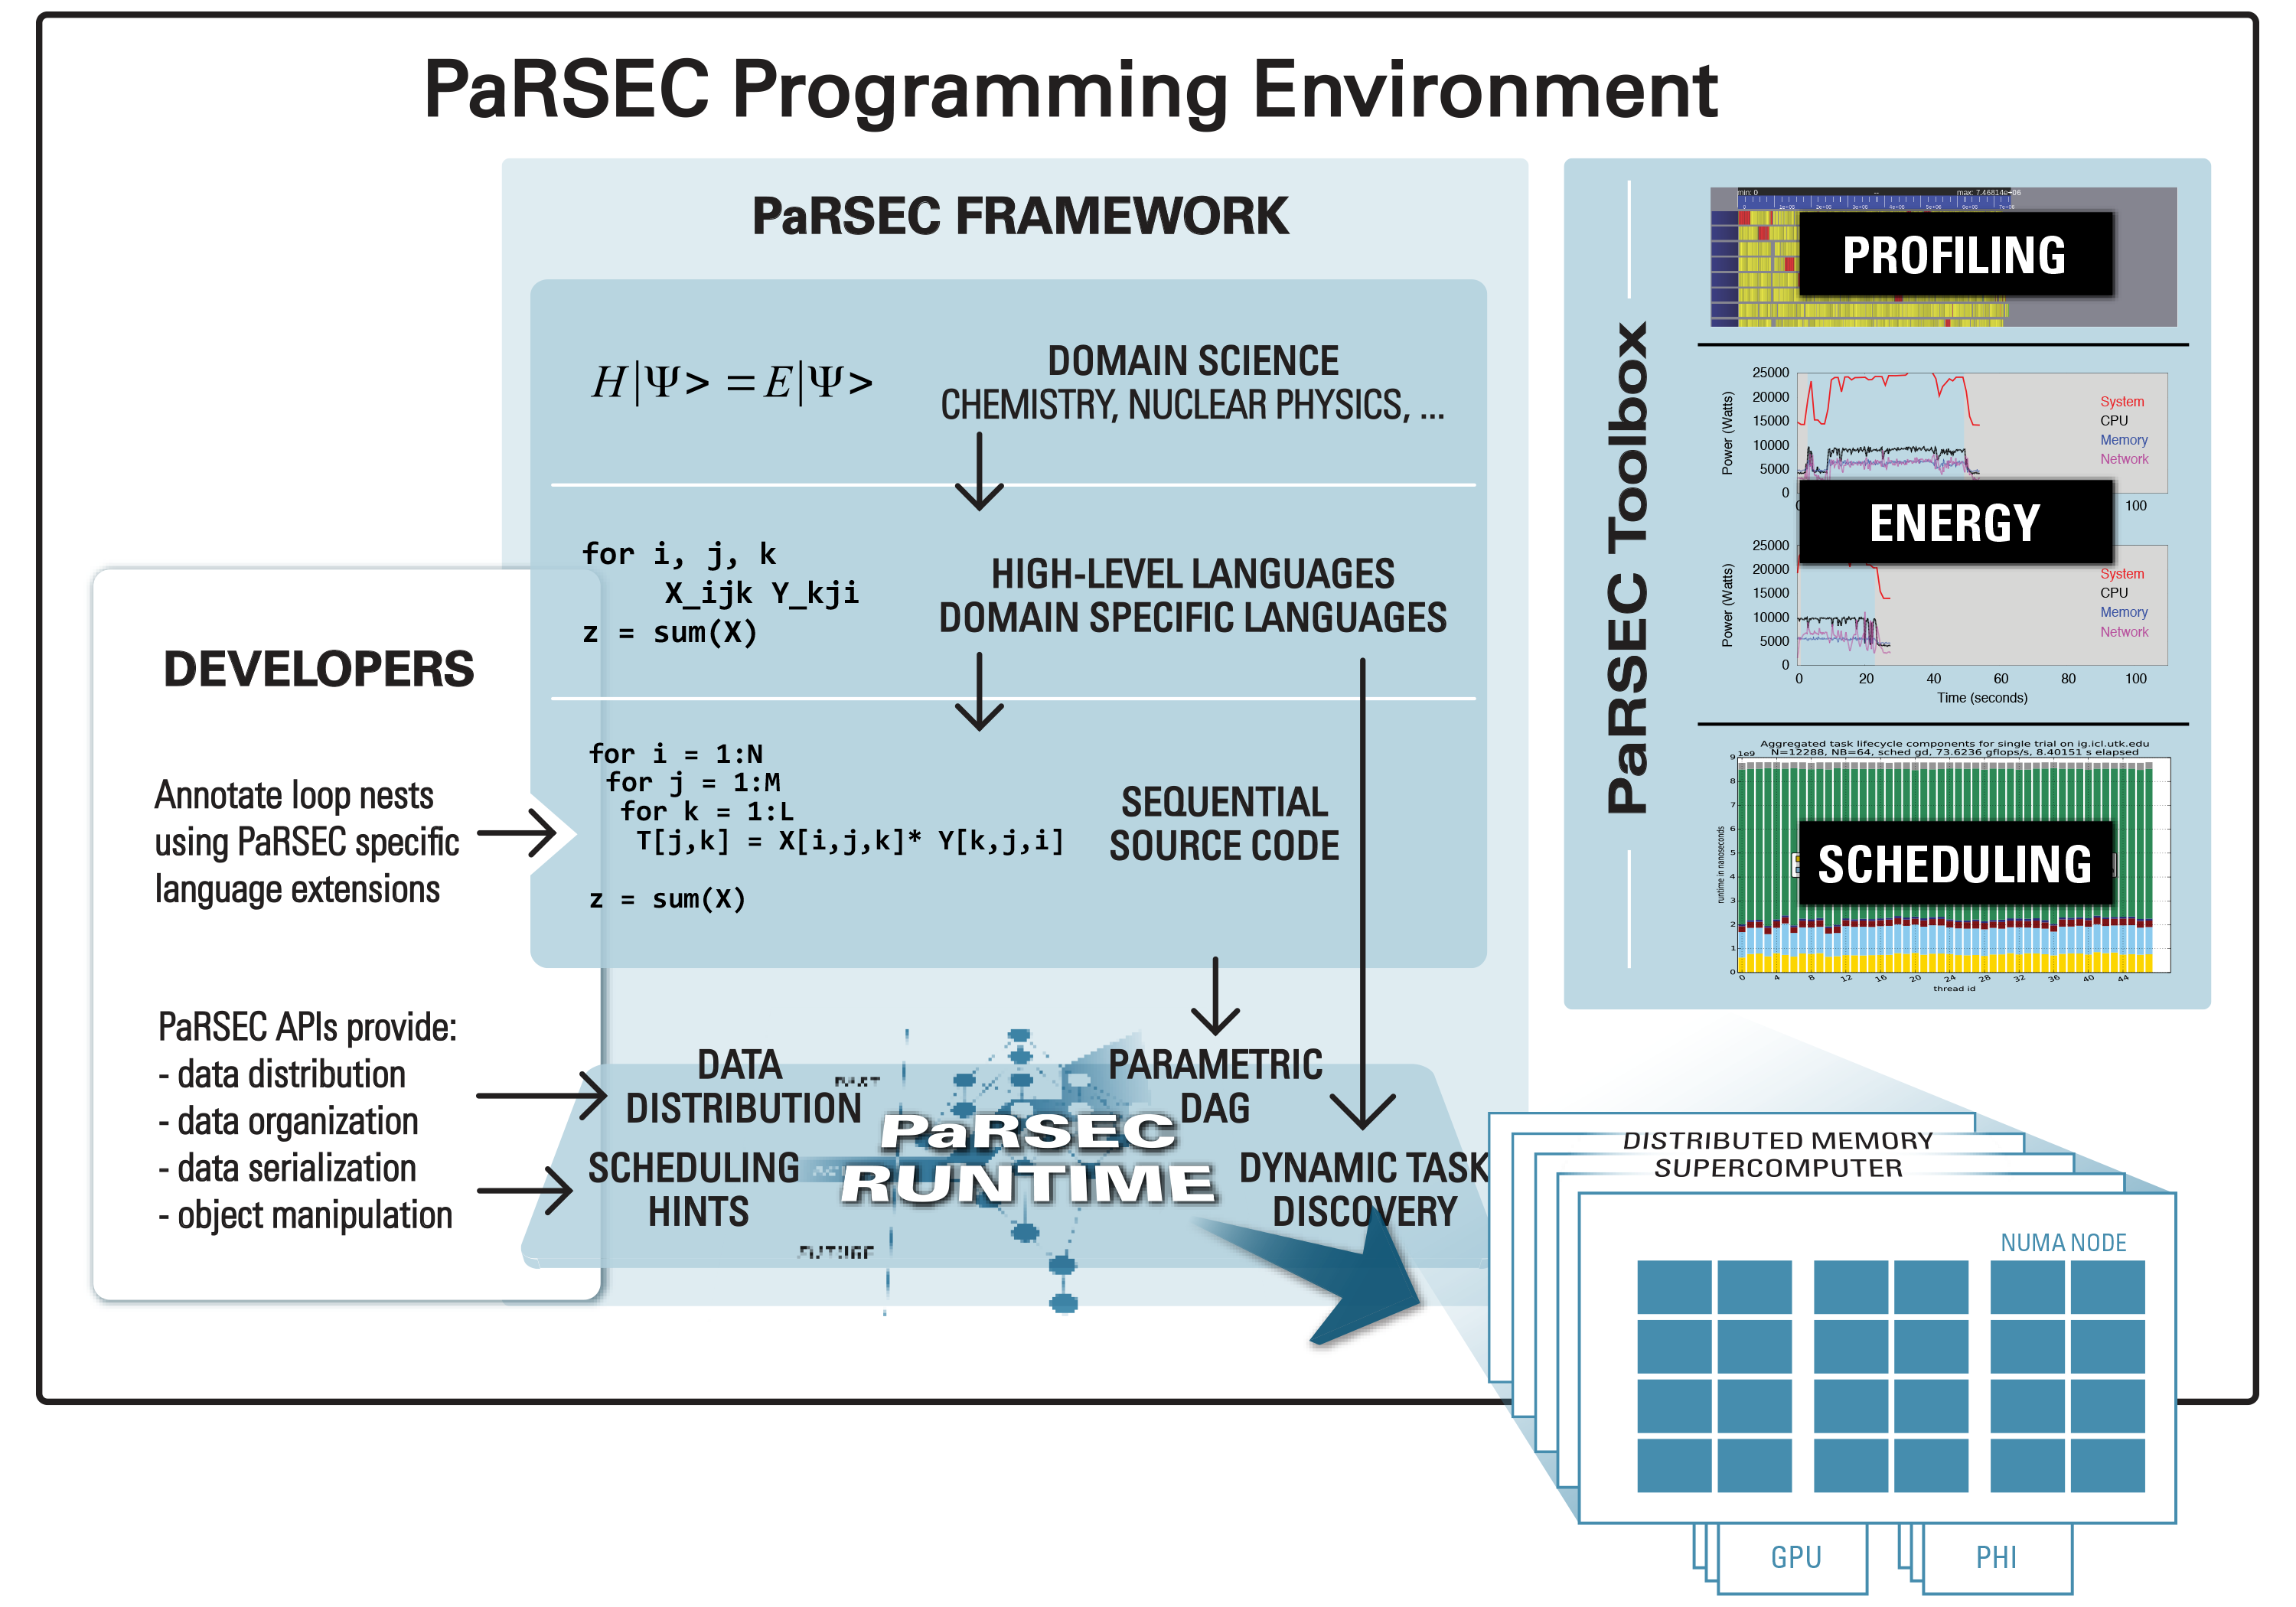
\includegraphics[scale=0.4]{projects/2.3.1-PMR/2.3.1.09-ParSEC/PaRSEC-diagram.png}
  \caption{PaRSEC architecture\label{fig:parsec}}
\end{wrapfigure}
%
PaRSEC is an open source, community-based implementation of a generic task-based
runtime that is freely available, and used by an increasing number of software
libraries. The PARSEC development team is mainly comprised of research staff at
UTK, but regular contributions from the community are provided via our presence
on GitHub and Bitbucket The project focuses on prototyping different
approaches to define task-based languages that will be able to exploit the full
range of capabilities of Exascale platforms. Without such a project, and based
on the current state of task-based runtimes, potential users will be stuck
either in fixed programming boundaries, or with particular programming
languages. The DTE project provides means to maintain a high competitiveness in the
field leading to more innovation on addressing the challenges we are facing
toward scalable, performant and Exascale ready programming paradigms.

\paragraph{Key  Challenges}
%\textit{Describe what is hard to do, why it is challenging.}

As we approach Exascale, a number of aspects of the hardware and software
environment pose challenges. First and foremost, keeping pace with the
architectural changes on current and future machines requires changes not only
on how we take advantage of the hardware capabilities, but how we reshape our
algorithms and applications to expose enough parallelism to maximize the use of
the underlying hardware. The number of nodes, threads per node, memory
hierarchies and support for increased computational capabilities (accelerators)
will continue to increase, while the currently available programming paradigms
are still struggling with parallelism at the node level.

\paragraph{Solution Strategy}
%\textit{Describe your basic strategy for addressing the challenges.}
The approach followed in PaRSEC is to provide a low-level, flexible and dynamic
runtime able not only to schedule tasks at the node level, but to handle data
transfers between different memory (both inter and intra nodes), memory
hierarchies, heterogeneous architectures with support for accelerators with a
simple programming scheme. The proposed approach envisions a middle-ground
solution, addressing both hardware and software challenges. At the hardware
level a team of dedicated developers extends PaRSEC to map it's capabilities to
the hardware and to improve it's scalability and performance. At the upper level
the interaction with the users is through building Domain Specific Languages
with the target domain scientists in mind, that will facilitate the expression
of algorithmic parallelism with familiar constructs mapped on the exposed low-level
capabilities.

\paragraph{Recent Progress}
% \textit{Describe what you have done recently.  It would be good to have some
% kind of figure or diagram in this section.}
The runtime system of PaRSEC has been extended to provide a better support of
dynamic task pools (DAGs of tasks), opening the runtime to new classes of
algorithms, such as those where the total number of tasks is a priori unknown.
% Some target applications (typically from NWChemEx) produce a dynamic DAG of
% tasks, for which the runtime cannot predict at the initialization time how many
% tasks exist, and where they will be executed.
We enabled such dynamic DAGs by removing internal constraints on how tasks are
identified and how dependencies are tracked. However, one of the missing
capabilities, the detection of the application termination, needed to be
provided explicitly.
% to determine termination of the DAG, the user had to provide the termination
% detection in a task, and broadcast explicitly that termination to all the nodes.
We added a set of termination detection algorithms to remove this step with
better efficiency, and providing a complete solution to handling dynamic DAGs.


An important aspect of the DTE project is to define and prototype scalable
domain specific languages that enable a productive expression of parallelism for
end-user communities. PaRSEC presents multiple programming interfaces
(Parameterized Task Graphs for maximum parallelism, the popular serial task
insertion dataflow model to provide direct access to the runtime). In addition
the DTE team is in close contact with application teams to define parallel
abstractions that are suitable for their domain usage. Notably, the PaRSEC team
has ongoing collaboration with the SLATE linear algebra package and NWChemEx
chemistry package teams.
The PaRSEC development team did the first step toward the integration
of their framework into the SLATE (2.3.3.09) in the context of the
shared milestone (STPM11-23). The first prototype of the application
ran in a distributed environment and showed the capability of the
SLATE library using a modern fully capable runtime system. This work
involved enhancing the insert task interface available in the ParSEC
runtime to map onto the logic of a SLATE algorithm.

\begin{wrapfigure}{l}{.5\linewidth}
  \centering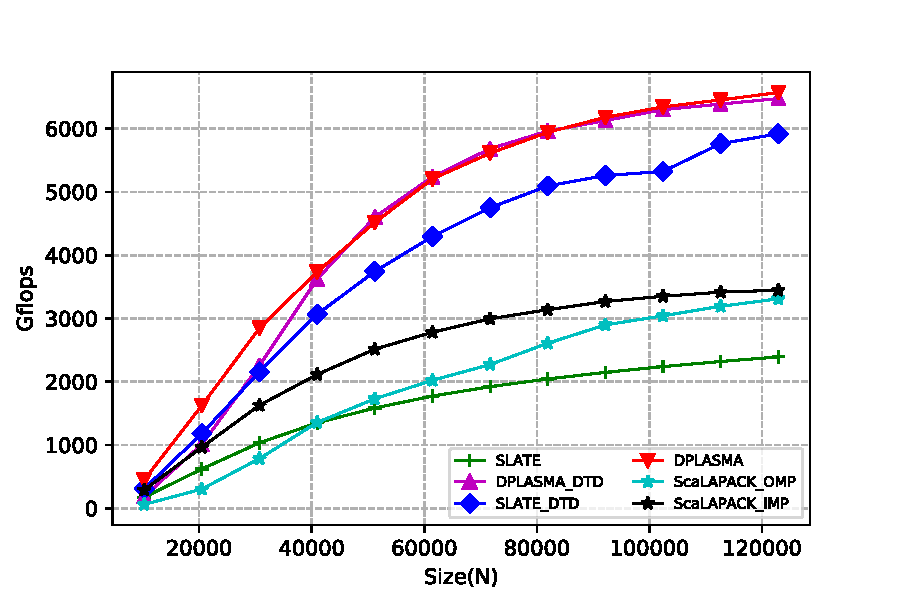
\includegraphics[scale=0.5]{projects/2.3.1-PMR/2.3.1.09-ParSEC/SLATE_inital_result_phicluster_scalapack.pdf}
  \caption{PaRSEC architecture \label{fig:slate-parsec}}
\end{wrapfigure}
%
In figure~\ref{fig:slate-parsec}, we compare the integration of SLATE
and PaRSEC against the state of the art. First against the two legacy
domain specific languages that have the capability to do linear
algebra; then against the regular SLATE using OpenMP for intra-node
parallelism, and MPI for communication; and finally against ScaLAPACK,
which is the reference for distributed linear algebra.

On the software quality side, the PaRSEC runtime has been evaluated and amended
to compile and run on all major target pre-Exascale platforms (ALCF Mira, Theta; OLCF
Titan, Summit-dev). In particular the detection of architecture specific
features on NVIDIA V100 accelerators and Power processors has been improved.
PaRSEC now includes a Spack definition file to ease the deployment on future
target systems as part of the system software SDK effort.

\paragraph{Next Steps}
%\textit{Describe what you are working on next.}

% GPU engine
A major effort at refactoring the accelerator and GPU component
of the PaRSEC runtime is ongoing. The new runtime component handles
memory transfers to/from accelerators as schedulable completion events
that can trigger asynchronously the next step of the accelerated task
and/or dependent tasks. The new engine is modular, one of the component
provides a CUDA backend optimized for NVIDIA accelerators, and a new component
will provide an OpenMP target backend for portability to other hardware.


We are improving the performance characterization system of PaRSEC to
enable users to get detailed information on the performance of their
applications that use PaRSEC as a runtime system. Part of this effort
is shared with the development of Software Defined Events in ExaPAPI
and the integration within the PaRSEC runtime.

% Task cancellation
The PaRSEC runtime will be augmented with the capability for any task
to decide that a given algorithm has no more reason to be
executed. This feature requires the runtime to properly remove any
trace of the algorithm without going into extreme solutions. We do not
want to dry run the algorithm without actually executing anything, and
we do not want to remove the task from the runtime without any
consideration for the other nodes. The solution will have to be a
local decision that will leave the runtime in a coherent state without
impeding the performance with the execution of useless tasks.


% Collective API
The detection of collective pattern at the runtime level is a hard
problem.  To enhance the insert task interface, the PaRSEC development
team will provide a communication API. It will give the developer the
capability to express communication where and when it seems fit during
the algorithm.